\section{Background: What is Serialism?}

%History of Serialism -- when, who
In general, serialism is a musical composition technique where a set of values, chosen through some methodical process,
generates a sequence of musical elements. Its origins are often attributed to Arnold Schoenberg's twelve-tone technique, which
he began to use in the 1920s. In this system, each note in the chromatic scale is assigned an integer value, giving us a set of twelve
"pitch classes" (see fig. 1).
%Description of technique -- pitch classes, specific orderings as basis for melody, harmony

Schoenberg's method then takes each of these integers, and orders them into a $twelve$ $tone$ $row$, where each number appears
exactly once. We refer to this row as the $prime form$ of a piece, and conventionally refer to it as $P_0$. The
composer can then generate other rows that are derived from $P_0$ through three types of transformations: transposition, inversion, and retrograde. In each of these transformations, we always use mod 12 arithmetic to preserve the numbering system of our pitch classes. Transposing a row consists of taking each pitch class in the row and adding the same number to each. If we transpose $P_0$ by four semitones, we add four mod twelve to each pitch class in $P_0$ and end up with a new row called $P_4$. In general, $P_x$ is a transposition of $P_0$ by $x$ semitones. To invert a row, we flip each interval between two pitch classes in that row. For example, if $P_0$ starts with pitch classes 0-4-1, then we have an interval of +4 between the first two pitches and -3 between the second two. In the inverse of $P_0$ (called $I_0$), the first interval would be -4 and the second would be +3, giving us 0-8-11 as our first three pitch classes. The subscript of $I_x$  refers both to the number of transpositions required to arrive at $I_x$ from $I_0$, and to the prime row $P_x$ that would need to be inverted to generate $I_x$. The final row operation is a retrograde transformation, which merely consists of reading a row backwards. That is, $R_x$ is generated by reading the pitch classes of $P_x$ in their opposite order. One can also have a retrograde inversion; $RI_x$ is generated by reading the pitch classes of $I_x$ backwards.

Once a composer chooses a $P_0$, these three transformations can be applied to varying degrees to generate a $twelve$ $tone$ $matrix$, which will contain each $P$ row as a row in the matrix and each $I$ row as a column. Furthermore, all of the $R$ and $RI$ rows are found by reading the rows in the matrix from right to left or the columns from bottom to top, respectively. An example of a twelve tone matrix from one of Shoenberg's pieces can be found below (fig. 2).
%Possible transformations
%Notation


\begin{figure}
\begin{center}
\resizebox{6in}{!}{\includegraphics*{figures/hello}}
\end{center}

\caption{Hello eps\label{m42}}
\end{figure}


%\begin{figure} % use float package if you want it here
%  \centering
%  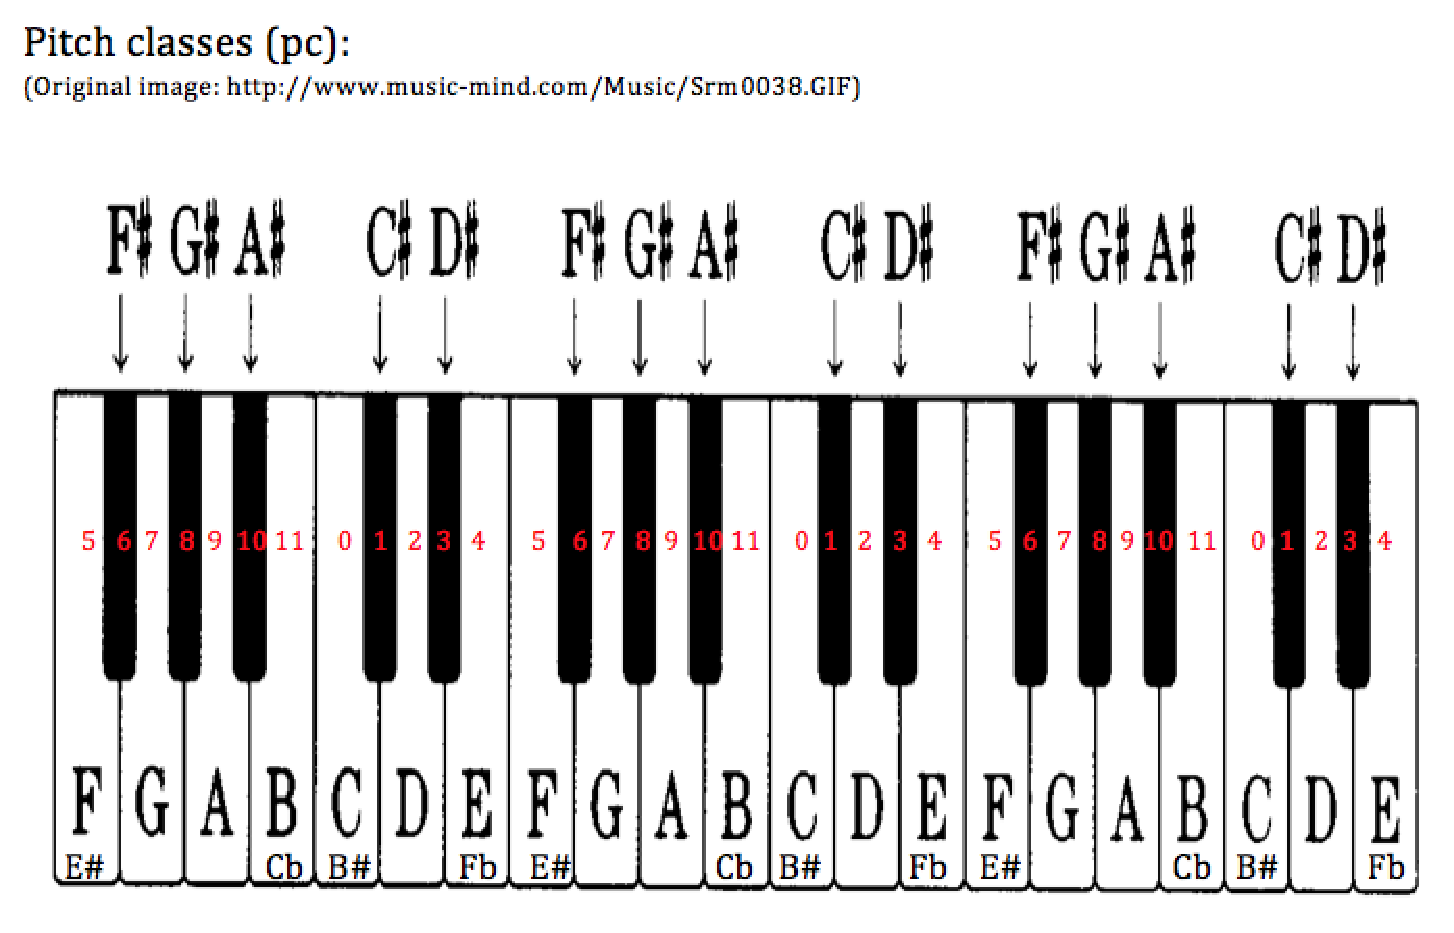
\includegraphics[width=10cm]{figures/serialismPianoImage}
%  \caption{The second picture}
%  \label{fig:xfig1}
%\end{figure}


